\begin{figure*}[htbp]
    \centering
    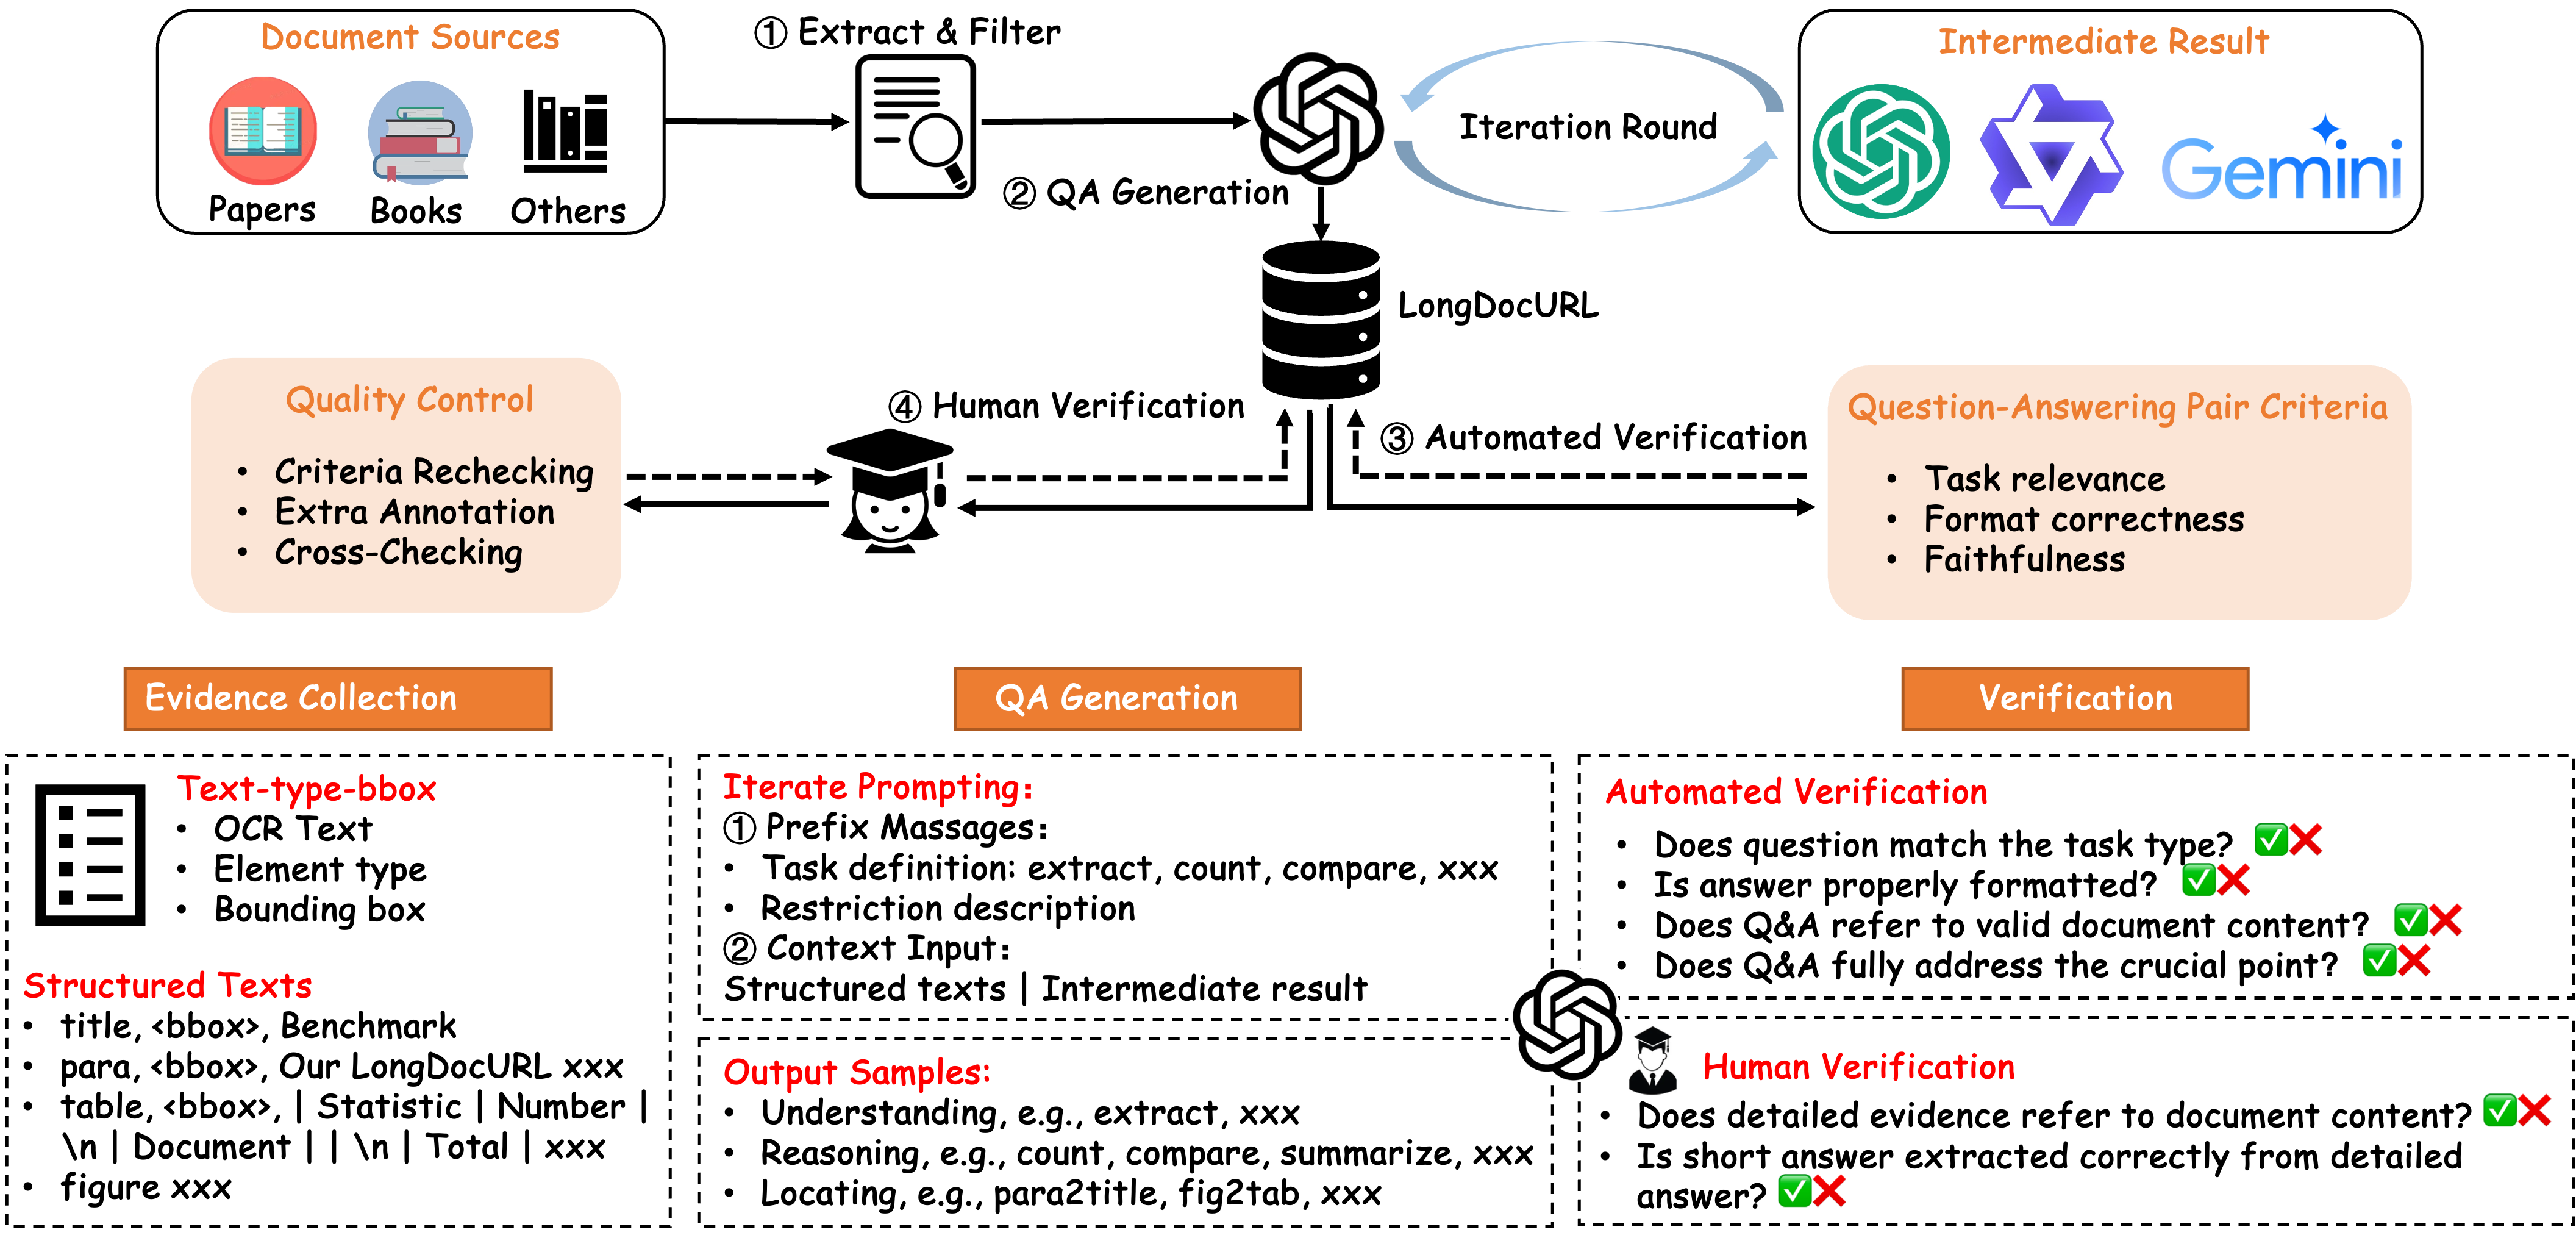
\includegraphics[width=\textwidth]{img/pipeline_1216.png} % 调整宽度
    \vspace{-0.3cm}
    \caption{Overview of our semi-automated construction pipeline. The pipeline comprises four modules: (a) \emph{Extract \& Filter}; (b) \emph{QA Generation}; (c) \emph{Automated Verification}; (d) \emph{Human Verification}.}
    \vspace{-0.2cm}
    \label{fig:pipeline}
\end{figure*}


\section{\benchName}
\label{sec:benchmark}

\subsection{Overview}
\label{subsec:overview}

Firstly, each question-answering pair can be categorized by three primary tasks: \emph{Understanding}, \emph{Reasoning}, and \emph{\Locating}, as discussed in \Cref{sec:intro}. Secondly, we define four types of answer evidences based on element type: (1) \emph{Text}: pure texts, such as paragraph; (2) \emph{Layout}: text elements with special layout meaning (generalized text), such as title, header, footer, table name and figure name; (3) \emph{Figure}: including charts and general images. (4) \emph{Table}. In addition, each question-answering pair can be classified into \emph{single-page} or \emph{multi-page} based on the number of answer evidence pages and \emph{single-element} or \emph{cross-element} based on the number of types of evidence elements. Based on different primary tasks and answer evidences, we divide our dataset into 20 sub-tasks. As shown in \Cref{fig:task_classification_and_distribution}, for the \emph{Understanding} or \emph{Reasoning} task, we divide our dataset into 8 sub-tasks according to the number of answer evidence pages. Compared to the two tasks, we pay more attention to the interrelations
among different types of elements in the \emph{Locating} task and we build 4 sub-tasks based on the combination of different element types. Data examples are presented in \Cref{xsec:data_examples}.

\subsection{Q\&A Construction}

\subsubsection{Evidence Collection}
\label{subsubsec:evidence_collection}
To objectively evaluate LVLM long document question-answering comprehension ability, we first crawl 200k PDF-formatted documents from CommonCrawl\footnotemark[1] and filter them by page length(\ie, 50\textasciitilde 150) and language(\ie, English) to create a candidate set of approximately 3,000 documents. Then, we categorize these candidates by document type. Specifically, we randomly select 5\textasciitilde10 pages from a document, and prompt GPT-4o to classify its document type based on document content and layout. We finally retain 396 documents to construct our benchmark. These documents span eight types: \emph{research reports \& papers}, \emph{user manuals \& guides}, \emph{books \& e-books}, \emph{theses \& dissertations}, \emph{work \& project summaries}, \emph{presentation materials}, \emph{project proposals}, and \emph{meeting minutes \& summaries}, with an average of 85.6 pages per document.

\footnotetext[1]{https://corp.digitalcorpora.org/corpora/files/CC-MAIN-2021-31-PDF-UNTRUNCATED/}

Thereafter, we utilize both PyMuPDF\footnotemark[2] and Docmind\footnotemark[3] to parse the PDF and extract texts and layout information from the documents. For instance, the tables are converted into markdown format with Docmind. We organize the extracted results in the format of \emph{\textbf{text-type-bbox}} triples as a symbolic representation of elements: 1) \emph{\textbf{text}}: the recognized text of the elements; 2) \emph{\textbf{type}}: the element type. 3) \emph{\textbf{bbox}}: the bounding box of the element. Notably, we build the element triples at the region level, such as paragraph, table, chart, footnote and title, instead of the line level.

\footnotetext[2]{https://pymupdf.readthedocs.io}
\footnotetext[3]{https://www.aliyun.com/product/ai/docmind}

\subsubsection{Q\&A Generation}
\label{Data Generation}

Directly prompting LVLM to generate conversational question-answering pairs based on a single or multiple document images proves often ineffective, due to the inability to fully parse diverse elements present in the documents. Similar to LLaVA~\cite{LLaVA}, we adopt a two-stage pipeline: Initially, we parse our PDF-formatted documents and get the ``text-type-bbox'' triples discussed in \Cref{subsubsec:evidence_collection}. Subsequently, we design prompts to query LLMs/LVLMs in a multi-step round, and finally generate question-answering pairs. Specifically, as shown in \Cref{fig:pipeline}, we present the definition of each task and description of related restriction as a part of the prompts. Details can be found in \Cref{xsec:method_details}.

\subsection{Q\&A Verification}
\label{subsec:qa_verify}
\subsubsection{Automated Verification}
\label{subsubsec:auto_verify}
We design an automated method to verify the quality of synthesized question-answering pairs to identify and correct corresponding issues.
As shown in \Cref{fig:pipeline}, a qualified question-answering pair should be verified using these criteria: (1) \textbf{Task Relevance}. (2) \textbf{Format Correctness}. (3) \textbf{Faithfulness}.

\begin{table}[t]
    \centering
    \resizebox{0.45\textwidth}{!}{
            \begin{tabular}{lc}
            \toprule
            \textbf{Statistic} & \textbf{Number} \\
            
            \midrule
            \textbf{Document} \\
                ~- Total & 396 \\
                ~- Type & 8 \\
                ~- Avg. pages & 85.6 \\
              
            \midrule
            \textbf{Question \& Answer} \\
                ~- Total & 2,325 \\
                ~- Avg. question tokens & 35.5 \\
                ~- Max. question tokens & 277 \\
            \midrule
            \textcolor{gray}{Task Type} \\
                ~- Understanding & 1,243 (53.5\%) \\
                ~- Reasoning & 387 (16.6\%)  \\
                ~- \Locating & 695 (29.9\%) \\

            \midrule
            \textcolor{gray}{Type of Evidence Element} \\ 
                ~- Pure-text & 994 (42.8\%) \\
                ~- Layout & 779 (33.5\%) \\
                ~- Table & 556 (23.9\%) \\
                ~- Figure & 871 (37.5\%) \\

            \midrule
            \textcolor{gray}{Number of Evidence Pages} \\
                ~- Single-page question & 1,093 (47.0\%) \\
                ~- Multi-page questions & 1,230 (52.9\%)  \\
                ~- Unanswerable questions & 2 (0.1\%) \\

            \midrule
            \textcolor{gray}{Number of Evidence Element Types} \\
                ~- Single-element question & 1,463(62.9\%) \\
                ~- Cross-element question & 862(37.1\%) \\

            \midrule
            \textcolor{gray}{Answer Format} \\ 
                ~- String   & 941 (40.5\%) \\
                ~- Integer  & 431 (18.5\%) \\
                ~- Float & 185 (8.0\%) \\
                ~- List & 757 (32.6\%) \\
                ~- None & 11 (0.5\%) \\
            \bottomrule
        \end{tabular}}
        \captionof{table}{Document and Q\&A statistics based on different tasks and answer evidences.}
        \vspace{-0.5cm}
        \label{tab:statistics}
\end{table}

\begin{figure}[t]
    \centering
    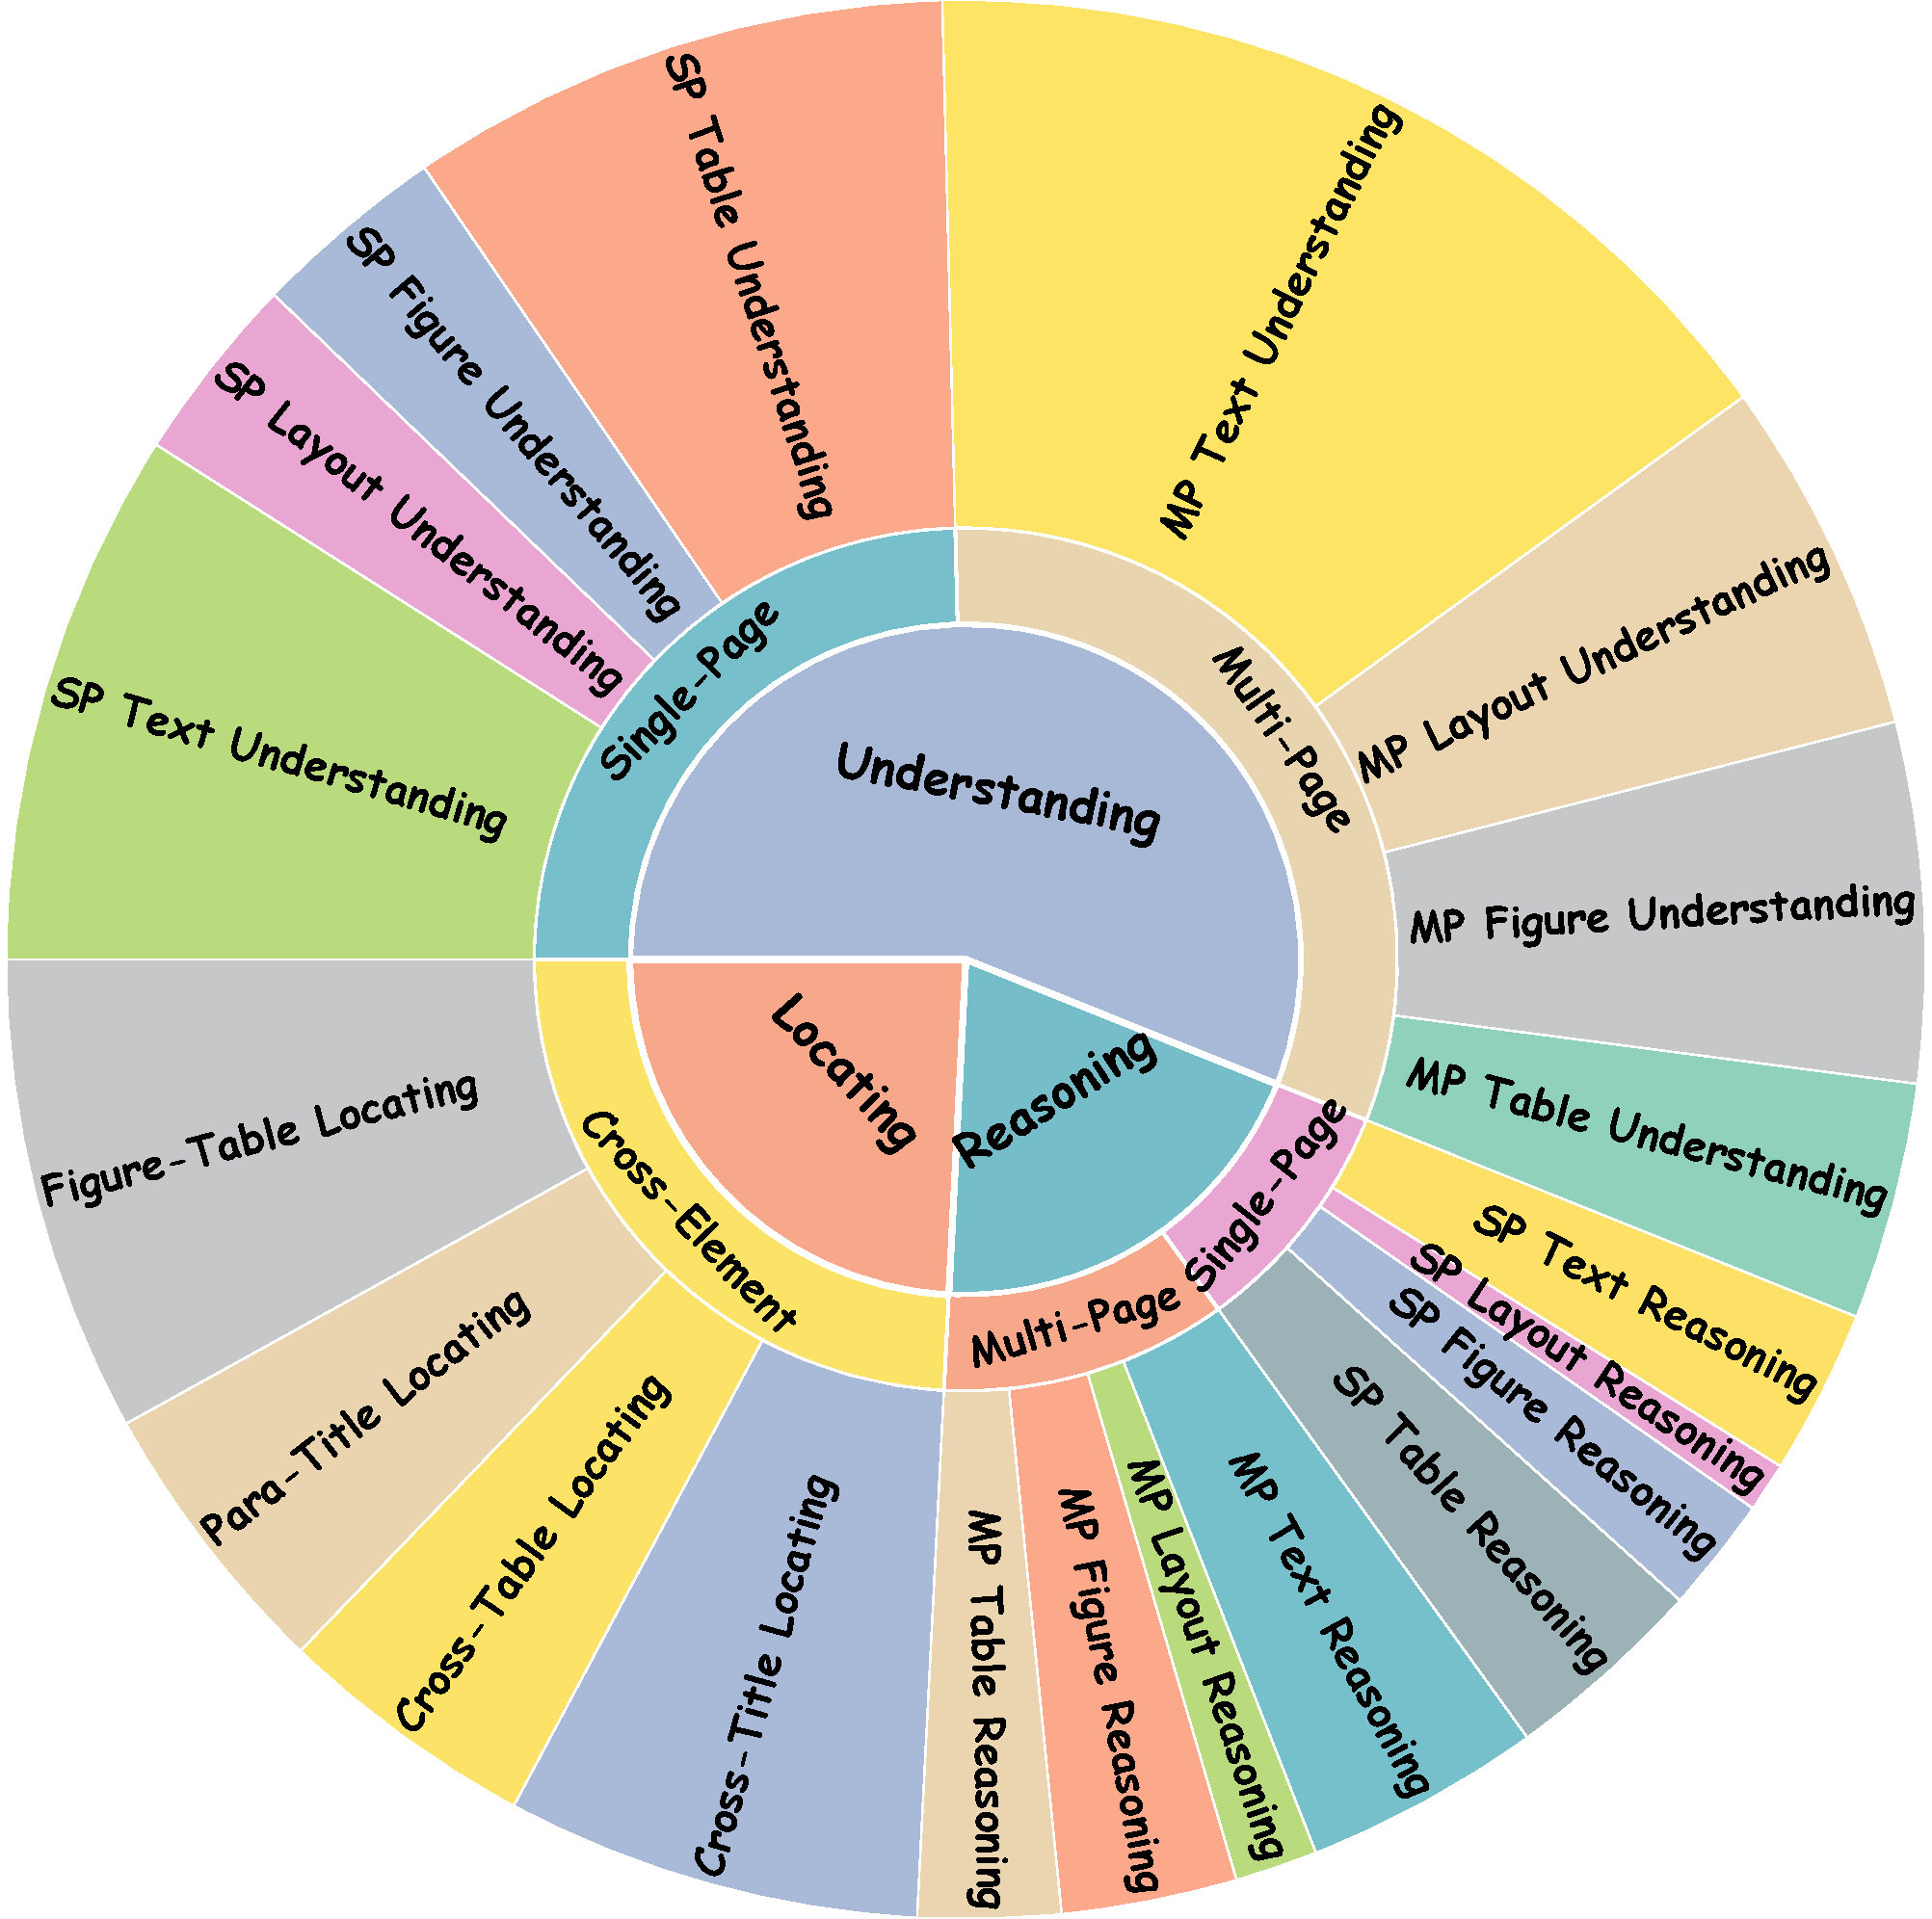
\includegraphics[width=0.4\textwidth]{img/circle_percentage.pdf} % 调整宽度
    \caption{Our \benchName~comprises 20 sub-tasks. \textbf{Inner}: divided by the primary task categories (Understanding, Reasoning, and \Locating). \textbf{Middle}: divided by the number of answer evidence pages (Single-Page, Multi-Page), and the number of types of evidence elements (Cross-Element). \textbf{Outer}: divided by the types of evidence elements (Text, Table, Figure, Layout).}
    \vspace{-0.5cm}
    \label{fig:task_classification_and_distribution}
\end{figure}

The verification results are utilized to classify samples: those that fail are marked as negative, and those that pass are marked as positive.
We analyze the verification results and observe approximately 75.2\% of the raw data in the Cross-Title \Locating~task are marked as negative samples, while the percentage is 19.6\% in the Cross-Table \Locating~task. Additional statistics data is presented in \Cref{tab:qa_numeric_verification}. In the next stage (\Cref{subsubsec:human_verify}), we present both the final result and texts of verification chains to the human annotator as reference information to guide further verification.


\subsubsection{Human Verification}
\label{subsubsec:human_verify}
There are two shortcomings of automated verification in \Cref{subsubsec:auto_verify}: (1) It only completes the classification of positive and negative samples, but does not recycle them, which causes waste. (2) When verifying the consistency between the question-answer pair and the document, only the text information is referenced, which may lost significant visual structure information compared to the source document. In the human verification stage, we focus on tasks that are challenging for automated verification, such as recovering negative samples and checking the consistency between the question-answering pair and the visual source information. The Human Verification module comprises the following parts: 

\begin{itemize}[leftmargin=*]
    \item \textbf{Criteria Rechecking.} The annotator reviews the intermediate process of machine verification to determine whether it is reasonable and whether the negative samples can be recovered by simply correcting the question-answer pair.
    \item \textbf{Extra Annotation.} Human annotators should oversee the question-answer pair process using the source visual document, not the parsed one. First, they need to verify if the evidence provided by the model aligns with the document's content, and then ensure that the final answer can be derived step by step from the intermediate process.
    \item \textbf{Cross-Checking.} After the annotators complete the first round of annotation, we require the annotators to cross-check each other's annotation results to improve the quality of annotation.
\end{itemize}

The labor resource allocation for data annotation is detailed in \Cref{xsec:labeling_labor}.


\subsection{Dataset Statistics}
\label{Dataset Statistics}

As shown in \Cref{tab:statistics} and \Cref{fig:document_distribution}, our \benchName~comprises 396 documents and 2,325 question-answering samples. The average pages per document range from 50 to 150. The cross-element locating task we designed contributes 37.1\% of the data, providing support for evaluating the model's cross-element interaction capabilities in long contexts. The dataset includes five types of answers, ensuring compatibility with automated evaluation while maintaining completeness and accuracy. In addition, we compare the characteristics of question set in our \benchName~with that in MMLongBench-Doc. The results are presented in \Cref{xsec:comparison_with_mmlongbenchdoc}.


